\newpage
\section{Boundary Value Problem for the Laplace Equation}

\subsection{The Dirichlet and Neumann Problems}

Last time, we were looking at the Laplace equation
$$
-\Delta u=f \quad \text { in } \mathbb{R}^{n}
$$
We saw a few ways to look at this:
\begin{itemize}
    \item via the fundamental solution. This led to elliptic regularity.
    \item via the maximum principle. This gave us a way to prove uniqueness of solutions.
    \item via energy estimates. This is what we will discuss today.
\end{itemize}

When we look at the Laplace equation, we need some boundary behavior? The \textbf{Dirichlet problem} is to solve the Laplace equation with the following boundary condition.
$$
\begin{cases}-\Delta u=f & \text { in } \Omega \subseteq \mathbb{R}^{n} \\ u=g & \text { on } \partial \Omega\end{cases}
$$
Alternatively, we can look at the \textbf{Neumann problem} with a boundary condition on the normal derivative of the solution.
$$
\begin{cases}-\Delta u=f & \text { in } \Omega \subseteq \mathbb{R}^{n} \\ \frac{\partial u}{\partial \nu}=g & \text { on } \partial \Omega\end{cases}
$$
Can we impose both the Dirichlet and Neumann boundary conditions? The answer is not always. The equation
$$
\begin{cases}-\Delta u=f & \text { in } \Omega \subseteq \mathbb{R}^{n} \\ u=g_1 & \text { on } \partial \Omega \\ \frac{\partial u}{\partial \nu}=g_2 & \text { on } \partial \Omega\end{cases}
$$
is an overdetermined problem. It makes sense to consider this locally.
\begin{figure}[H]
    \centering
    
\includegraphics[width=0.5\textwidth]{Pics/23-1.png}
\end{figure}
This local problem will in general have uniqueness but not necessarily existence. This leads to a type of problem called a \textbf{unique continuation problem.}

\subsection{Uniqueness concerns for the Dirichlet and Neumann problem}
\begin{proposition}
    [Uniqueness for the Dirichlet problem] 
     The solution to the Dirichlet problem
$$
\begin{cases}-\Delta u=f & \text { in } \Omega \subseteq \mathbb{R}^{n} \\ u=g & \text { on } \partial \Omega\end{cases}
$$
is unique.
\end{proposition}
\begin{proof}
    Suppose $u_{1}, u_{2}$ are solutions. Then $v=u_{1}-u_{2}$ solves
$$
\begin{cases}-\Delta v=0 & \text { in } \Omega \subseteq \mathbb{R}^{n} \\ v=0 & \text { on } \partial \Omega\end{cases}
$$
We want to show that $v=0$. We have
$$
\begin{aligned}
0 &=\int-\Delta v \cdot v d x \\
&=\int-\partial_{j} \partial_{j} v \cdot v d x
\end{aligned}
$$
Green's theorem gives
$$
=\int \partial_{j} v \dot{\partial}_{j} v-\int_{\partial \Omega} \frac{\partial v}{\partial \nu} \cdot \underbrace{v}_{=0} d \sigma
$$
So we get
$$
0=\int_{\Omega}|\nabla v|^{2} d x
$$
which tells us that $\nabla v=0$ in $\Omega$. Thus, $v$ is constant, and the boundary condition tells us that $v=0$.

\qed 
\end{proof}
\begin{remark}
     What about uniqueness of the Neumann problem?
    $$
    \begin{cases}-\Delta u=f & \text { in } \Omega \subseteq \mathbb{R}^{n} \\ \frac{\partial u}{\partial \nu}=g & \text { on } \partial \Omega\end{cases}
    $$
    By the same computation, we still get that
    $$
    \int_{\Omega}|\nabla u|^{2}=0
    $$
    which tells us that $u$ is constant. The boundary condition is satisfied by any constant, however. So solutions are unique modulo constants.
\end{remark}

\subsection{Existence using energy type estimates}
If $f: \mathbb{R} \rightarrow \mathbb{R}$, then a minimum point $x_{0}$ for $f$ must have $f^{\prime}\left(x_{0}\right)=0 .$ We can do the reverse. If we have an equation for a function, we can write it as the derivative of another function and interpret our equation as finding the minimizers (or critical points) for this function.
Looking at functions $u: \Omega \subseteq \mathbb{R}^{n} \rightarrow \mathbb{R}$, associate the functional
$$
\mathcal{L}(u)=\int_{\Omega}|\nabla u|^{2}-f \cdot u d x
$$
We will call this the \textbf{Lagrangian} of the problem. Our goal is to minimize $\mathcal{L}(u)$ over a good class of functions $u$; we can assume some nice regularity and our boundary condition. Let $\mathcal{A}=\left\{u: \Omega \rightarrow \mathbb{R} \mid u \in C^{2}, u=0\right.$ on $\left.\partial \Omega\right\}$. So we want
$$
\min _{u \in \mathcal{A}} \mathcal{L}(u)
$$
Does a minimum exist? We will not answer this today, but observe that $\mathcal{L}$ is strictly convex because it is the sum of a positive quadratic form and a linear term. If we have a minimum, then by strict convexity, the minimum will be unique.

We may also ask: What equation does a minimum satisfy? Suppose $u$ is a minimum. Take $v \in \mathcal{D}(\Omega)$, and set $u_{h}=u+h v$

\begin{figure}[H]
    \centering
    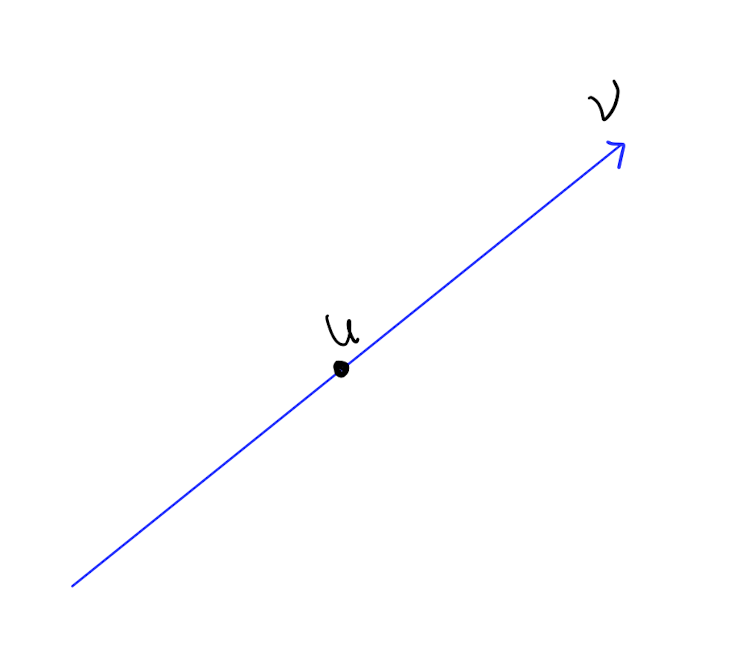
\includegraphics[width=0.3\textwidth]{Pics/23-2.png}
\end{figure}
Look at $\mathcal{L}\left(u_{h}\right)$ as a function of $h$. This has a minimum at $h=0$, which tells us that
$$
\frac{d}{d h} \mathcal{L}\left(u_{h}\right)=0 \quad \text { at } h=0
$$
Write
$$
\mathcal{L}\left(u_{h}\right)=\int|\nabla(u+h v)|^{2}-f \cdot(u+h v) d x
$$
so
$$
\left.\frac{\partial}{\partial h} \mathcal{L}\left(u_{h}\right)\right|_{h=0}=\int \nabla u \cdot \nabla v-f \cdot v d x
$$
Hence,
$$
0=\int \nabla u \cdot \nabla v-f \cdot v d x
$$
for all $v \in \mathcal{D}(\Omega)$. Integration by parts gives us
$$
\begin{aligned}
&=\int_{\Omega}-\Delta u \cdot v-f v d x \\
&=\int_{\Omega} v(-\Delta u-f) d x
\end{aligned}
$$
So we get
$$
-\Delta=f \quad \text { in } \Omega
$$
And we can append our favorite boundary condition.

\begin{remark}
The regularity condition $u\in\con^2$ is not the correct condition to use. Really, we want to use Soblev spaces, which we have not discussed yet.
\end{remark}

\subsection{Green's functions for domains with boundary} 
Circle back to the fundamental solution and try to use it in a domain with boundary. We will look at how this doesn't work and how it can be fixed. In $\mathbb{R}^{n}$, we have the formal computation
$$
\int-\Delta u \cdot K\left(x-x_{0}\right) d x=\int u \cdot-\underbrace{\Delta K}_{\delta_{x_{0}}}\left(x-x_{0}\right) d x
$$
If $-\Delta u=f$, then
$$
\int f \cdot K\left(x-x_{0}\right) d x=u\left(x_{0}\right)
$$
What about a domain with boundary?
$$
\int_{\Omega}-\Delta u \cdot K\left(x-x_{0}\right) d x=\int u \cdot-\Delta K\left(x-x_{0}\right) d x+\int_{\partial \Omega}-\frac{\partial u}{\partial \nu} \cdot K\left(x-x_{0}\right)+u \cdot \frac{\partial}{\partial \nu} K\left(x-x_{0}\right) d \sigma
$$
If $u$ solves the Dirichlet problem
$$
\begin{cases}-\Delta u=f & \text { in } \Omega \subseteq \mathbb{R}^{n} \\ u=g & \text { on } \partial \Omega\end{cases}
$$
then
$$
u\left(x_{0}\right)=\int_{\Omega} f(x) K\left(x-x_{0}\right) d x+\int_{\partial \Omega} \frac{\partial u}{\partial \nu} K\left(x-x_{0}\right)-g \cdot \frac{\partial K}{\partial \nu}\left(x-x_{0}\right) d \sigma,
$$
but we do not know what $\frac{\partial u}{\partial \nu}$ is. We do not have this information, and recall that if we do, then we have an overdetermined problem.

How do we fix this? Perhaps the fundamental solution is not the object we want to be looking at. Replace $K\left(x-x_{0}\right)$ by $G\left(x, x_{0}\right)$ to get

$$
\int_{\Omega}-\Delta u \cdot G\left(x,x_{0}\right) d x=\int u \cdot-G\left(x,x_{0}\right) d x+\int_{\partial \Omega}-\frac{\partial u}{\partial \nu} \cdot G\left(x,x_{0}\right)+u \cdot \frac{\partial}{\partial \nu} G\left(x,x_{0}\right) d \sigma
$$
We would like the properties
$$
\left\{\begin{array}{l}
-\Delta_{x} G\left(x, x_{0}\right)=\delta_{x_{0}}, \\
G\left(x, x_{0}\right)=0
\end{array} \quad x \in \partial \Omega\right.
$$

If we have these properties, then
$$
u\left(x_{0}\right)=\int_{\Omega} f \cdot G\left(x, x_{0}\right) d x+\int_{\partial \Omega} g \frac{\partial}{\partial \nu} G\left(x, x_{0}\right) d \sigma .
$$
If we had such a function $G$, then we could solve the Dirichlet problem. Call this function $G$ the \textbf{Green function} in $\Omega$.If we are solving the Neumann problem, we may get a different Green function.

\begin{remark}
    $G=G\left(x, x_{0}\right)$, not $G\left(x-x_{0}\right)$ because translation invariance is broken by our domain. If you translate the domain with boundary, you will not get the same domain.
\end{remark}

To find such a function $G$, we would try
$$
G\left(x, x_{0}\right)=K\left(x-x_{0}\right)+\psi\left(x, x_{0}\right)
$$
and look for an equation for $\psi$. We need
$$
\begin{cases}-\Delta_{x} \psi\left(x, x_{0}\right)=0 & \text { in } \Omega \\ \psi\left(x, x_{0}\right)=-K\left(x-x_{0}\right) & x \in \partial \Omega\end{cases}
$$
$K\left(x-x_{0}\right)$ is smooth for $x \in \partial \Omega$ and $x_{0} \in \Omega$, so by elliptic regularity, $\psi$ should be smooth. $\psi$ can be found by solving a Dirichlet problem.

\begin{remark}
    ~\
    \begin{itemize}
        \item  You may think this is leading us in a circle, but this is not the case: Here, we are solving a Dirichlet problem with a very special boundary data, $K\left(x-x_{0}\right)$. This may make the Green's function easier to find than solving the original equation otherwise.
        \item The Green function is symmetric:
        $$
        G(x, y)=G(y, x)
        $$
    \end{itemize}
\end{remark}

Let's calculate some Green's functions.

\begin{example}
    [Half-plane]
     Let $\Omega=\left\{x_{n}>0\right\} .$ The idea is to calculate $G$ using symmetries. Here is the picture we should have in mind:
     \begin{figure}[H]
         \centering
         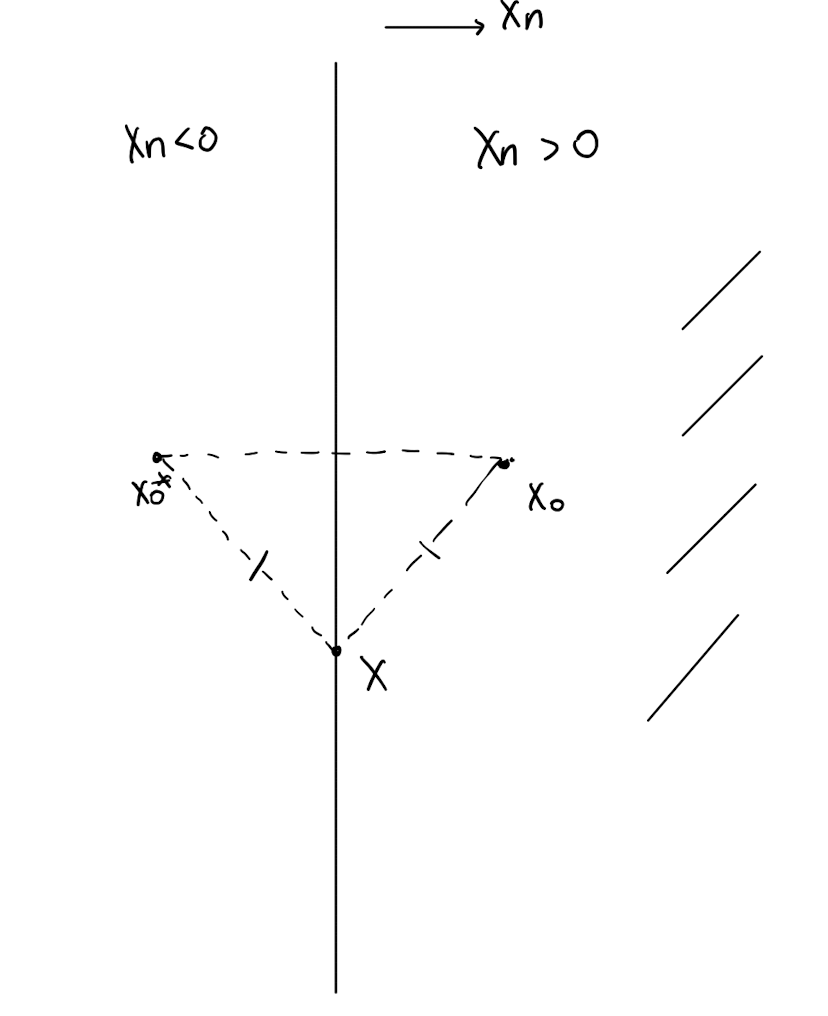
\includegraphics[width=0.5\textwidth]{Pics/23-3.png}
     \end{figure}
     We have
$$
G\left(x, x_{0}\right)=K\left(x-x_{0}\right)+\psi\left(x, x_{0}\right)
$$
If we were to use $x_{0}^{*}$, then $K\left(x-x_{0}^{*}\right)$ is harmonic in $\Omega$. Now also observe that for $x \in \partial \Omega$, $\left|x-x_{0}\right|=\left|x-x_{0}^{*}\right|$ for $x \in \partial \Omega$. Thus, the radial symmetry of $K$ gives $K\left(x-x_{0}\right)=K\left(x-x_{0}^{*}\right)$. This implies that we can choose
$$
G\left(x, x_{0}\right)=K\left(x-x_{0}\right)-K\left(x-x_{0}^{*}\right)
$$
\end{example}

\begin{example}
[Unit ball]
Let $\Omega=B(0,1)$. Here, we can try repeating the same argument but with inversion about the boundary of the circle:
\begin{figure}[H]
    \centering
    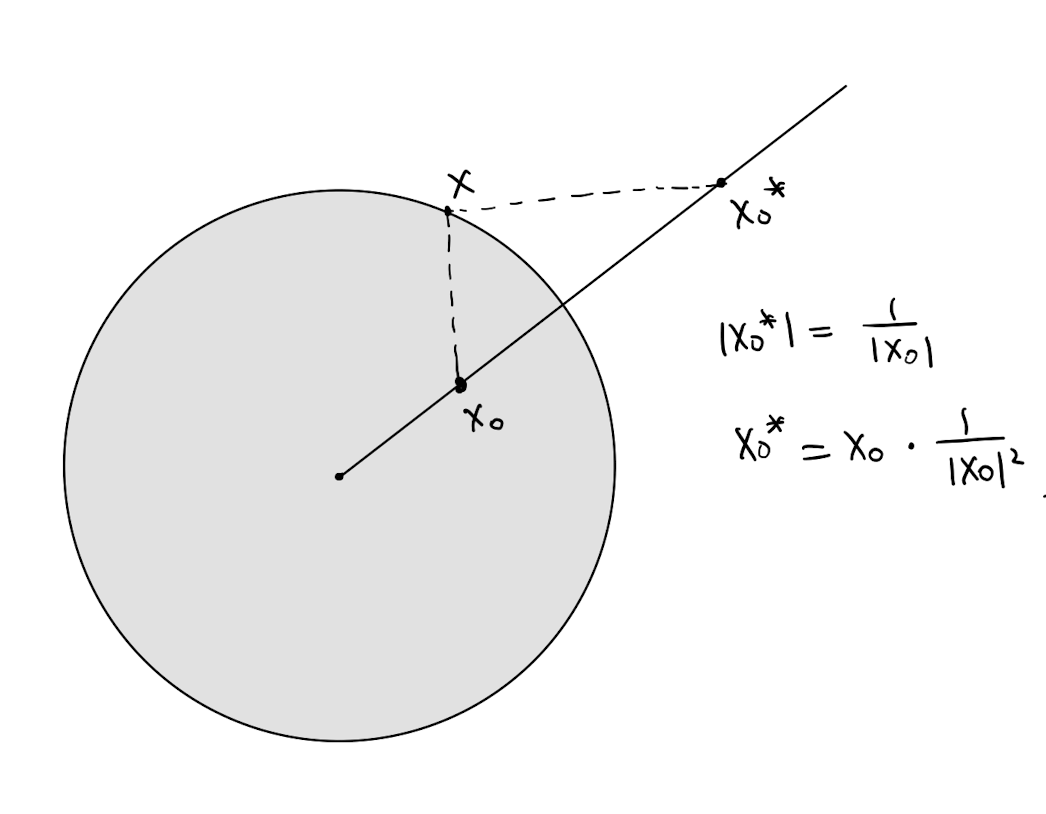
\includegraphics[width=0.5\textwidth]{Pics/23-4.png}
\end{figure}
If we have point $x \in \partial \Omega$, then
$$
\left|x-x_{0}\right|=\left|x-x_{0}^{*}\right| \cdot\left|x_{0}\right|
$$
So if we are in $\mathbb{R}^{n}$ for $n \geq 3$,
$$
G\left(x, x_{0}\right)=K\left(x-x_{0}\right)-|x_0|^{2-n} K\left(x-x_{0}^{*}\right)
$$
The proportionality constant comes from the fact that the first term is like $\left|x-x_{0}\right|^{2-n}$, while the second term is like $\left|x-x_{0}^{*}\right|^{2-n}$.

These kinds of computations are available only in very specific domains, so the existence of Green's functions is more of a qualitative question than a computational one.
\end{example}